\section{Von Neumann entropy}
    \subsection{Classical entropy}
        \begin{tcolorbox}[vert]
            For a random variable X, the entropy of X, $H\left(X\right) \approx $ amount of uncertainty: 
            \[H\left(X\right):= - \sum_{ i } p_i \log\left(p_i\right). \]
            $H\left(X\right)$ is maximized for the distribution over X that puts equal probabilities for all outcomes and is minimized if all its probability is on a single outcome.
        \end{tcolorbox}
    \subsection{Quantum entropy}
        \begin{tcolorbox}[vert]
            Let $\rho$ be a density matrix, its Von Neumann entropy is 
            \[S\left(\rho\right):= -Tr\left(\rho\log\left(\rho\right)\right).\]
        \end{tcolorbox}
        \begin{remark}{Remark}
            \begin{tcolorbox}[gris]
                Diagonal elements of $\rho$ are a classical probability distribution, $Tr\left(\rho\log\rho\right)$ means:
                \begin{itemize}[left=10pt, label=\textbullet]
                    \item write $\rho$ in its eigenbasis: $\rho=\sum_{ i }\lambda_i \ket{i}\bra{i}$, 
                    \item $-Tr\left(\rho\log\rho\right)=-\sum_{ n = 1 } ^{ d }\lambda_i \log\left(\lambda_i\right)$.
                \end{itemize}
            \end{tcolorbox}
        \end{remark}
        \noindent\textbf{Properties:}
        \begin{itemize}[left=10pt, label=\textbullet]
            \item $S\left(\rho\right) \geq 0$, 
            \item $S\left(\rho\right)$ is maximal for $\rho= \frac{\mathbbm{1}}{d}= \begin{pmatrix} \frac{1}{d} & \ldots & 0 \\ \ldots &  \ldots & \ldots \\ 0 & \ldots & \frac{1}{d} \end{pmatrix} $, 
            \item $S\left(\rho\right)=0 \iff \rho$ is a pure state $\iff \rho = \ket{\psi}\bra{\psi}$, 
            \item Concavity: $S\left(\alpha\rho_1+\left(1-\alpha\right)\rho_2\right) \geq \alpha S\left(\rho_1\right) + \left(1-\alpha\right)S\left(\rho_2\right)$.
        \end{itemize}
    \subsection{Entropy of a single qubit}
        For a single qubit, the density matrix is 
        \[\rho=\frac{1}{2}\left(\mathbbm{1}+\vec{a}\cdot \vec{\sigma}\right)=\frac{1}{2}\begin{pmatrix} \mathbbm{1}+a_z & a_x+ia_y \\ a_x-ia_y & \mathbbm{1}-a_z \end{pmatrix} , \mathspace \mathspace \mathspace \mathspace\left\|\vec{a}\right\| <1, \mathspace \vec{\sigma}= \left[\sigma_x \mathspace \sigma_y \mathspace \sigma_z\right].\]
        Then we can do a basis change $\rho \to \rho'$ such that $S\left(\rho\right)=S\left(\rho'\right)$ but $S\left(\rho'\right)$ is much easier to calculate. For this case, the basis change is 
        \[\rho'=\begin{pmatrix} \frac{1+\left\|\vec{a}\right\|}{2} & 0 \\ 0 & \frac{1+\left\|\vec{a}\right\|}{2} \end{pmatrix} .\]
        because $\lambda_{1,2}=\frac{1 \pm \left\|\vec{a}\right\|}{2}$. 
        \[\implies S\left(\rho\right)=S\left(\rho'\right)=H\left(\frac{1+\left\|\vec{a}\right\|}{2}, \frac{1-\left\|\vec{a}\right\|}{2}\right).\]
    \subsection{Compute a partial density matrix}
        \begin{tcolorbox}[vert]
            If overall state $\in \mathcal{H}_{AB}$ is $\rho_{AB}$ with $n_A= #$qubits in A and $n_B = #$qubits in B, then  
            \begin{align*} 
                \rho_A &= \sum_{ i \in \{0,1\}^{n_B} } \left(I_A \otimes \bra{i}_B\right) \rho_{AB} \left(I_A\otimes \ket{i}_B\right), \\
                \rho_B &= \sum_{ i \in \{0,1\}^{n_A}} \left(\bra{i}_A \otimes I_B\right) \rho_{AB} \left(\ket{i}_A \otimes I_B\right).
            \end{align*}
        \end{tcolorbox}
        \textbf{Special case: $n_A = n_B=1$},  $\rho_{AB}=$
        
        \begin{center}
        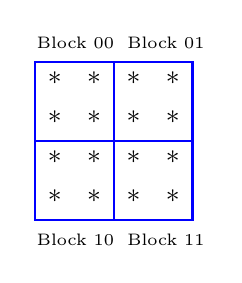
\begin{tikzpicture}
        \def\size{0.5} % taille d'une cellule
        \def\fs{6pt}     % taille de police pour les annotations
        
        % Dessin de la matrice 4x4 avec des *
        \foreach \i in {0,...,3} {
            \foreach \j in {0,...,3} {
            \node at (\j*\size, -\i*\size) {*} ;
            }
        }
        
        % Encadrement précis des blocs 2x2 (4 cellules par bloc)
        % Bloc haut-gauche (rouge)
        \draw[blue, thick]   (0-\size/2, 0+\size/2) rectangle (2*\size-0.5*\size, -2*\size+0.5*\size);
        % Bloc haut-droit (bleu)
        \draw[blue, thick]  (2*\size-0.5*\size, 0+\size/2) rectangle (4.5*\size-1*\size, -2*\size+0.5*\size);
        % Bloc bas-gauche (vert)
        \draw[blue, thick] (0-\size/2, -2*\size+0.5*\size) rectangle (2*\size-0.5*\size, -4*\size+0.5*\size);
        % Bloc bas-droit (orange)
        \draw[blue, thick](2*\size-0.5*\size, -2*\size+0.5*\size) rectangle (4.5*\size-1*\size, -4*\size+0.5*\size);
        \node[anchor=west, font=\fontsize{\fs}{\fs}\selectfont] at (-0.35, 0.5) {Block 00};
        \node[anchor=west, font=\fontsize{\fs}{\fs}\selectfont] at (\size + 0.3, 0.5) {Block 01};
        \node[anchor=west, font=\fontsize{\fs}{\fs}\selectfont] at (-0.35, -2) {Block 10};
        \node[anchor=west, font=\fontsize{\fs}{\fs}\selectfont] at (\size+0.3, -2) {Block 11};
        \end{tikzpicture} 
        \end{center}
        Then 
        \[\rho_A = \begin{pmatrix} * & * \\ * & * \end{pmatrix} = \begin{pmatrix} Tr\left(\text{Block 00}\right) & Tr\left(\text{Block 01}\right) \\ Tr\left(\text{Block 10}\right) & Tr\left(\text{Block 11}\right) \end{pmatrix} .\]
        This only works if we adopt the convention $ A \otimes B = \begin{pmatrix} A_{00}B & A_{01}B \\ A_{10}B & A_{11}B \end{pmatrix} $.
        \begin{remark}{Example}
            \begin{tcolorbox}[rouge]
               Let $\rho_{AB}=\ket{\psi_{Ab}}\bra{\psi_{AB}}$, where $\ket{\psi_{AB}}=\ket{0}_A \otimes \ket{+}_B$. Then 
               \[\rho_{AB}= \sigma_A \otimes \sigma_B \implies Tr_B\left(\rho_{AB}\right)=\sigma_A.\]
               Let's compute:
               \begin{align*} 
                   \ket{\psi_{AB}} &= \begin{pmatrix} 1 \\ 0 \end{pmatrix}_A  \otimes \frac{1}{\sqrt{2}}\begin{pmatrix} 1 \\ 1 \end{pmatrix}_B \\
                   \rho_{AB}&=\begin{pmatrix} 1 \\ 1 \\ 0 \\ 0 \end{pmatrix} \begin{pmatrix} 1 & 1 & 0 & 0 \end{pmatrix} \cdot \frac{1}{2} 
               \end{align*}
        \begin{center}
        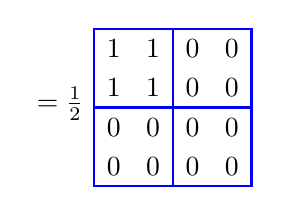
\begin{tikzpicture}
        \def\size{0.5} % taille d'une cellule
        \def\fs{6pt}     % taille de police pour les annotations
        
        % Dessin de la matrice 4x4 avec des *
        \foreach \i in {0,...,1} {
            \foreach \j in {0,...,1} {
            \node at (\j*\size, -\i*\size) {1} ;
            }
        }
        \foreach \i in {2,...,3} {
            \foreach \j in {2,...,3} {
            \node at (\j*\size, -\i*\size) {0} ;
            }
        }
        \foreach \i in {0,...,1} {
            \foreach \j in {2,...,3} {
            \node at (\j*\size, -\i*\size) {0} ;
            }
        }
        \foreach \i in {2,...,3} {
            \foreach \j in {0,...,1} {
            \node at (\j*\size, -\i*\size) {0} ;
            }
        }
        
        % Encadrement précis des blocs 2x2 (4 cellules par bloc)
        % Bloc haut-gauche (rouge)
        \draw[blue, thick]   (0-\size/2, 0+\size/2) rectangle (2*\size-0.5*\size, -2*\size+0.5*\size);
        % Bloc haut-droit (bleu)
        \draw[blue, thick]  (2*\size-0.5*\size, 0+\size/2) rectangle (4.5*\size-1*\size, -2*\size+0.5*\size);
        % Bloc bas-gauche (vert)
        \draw[blue, thick] (0-\size/2, -2*\size+0.5*\size) rectangle (2*\size-0.5*\size, -4*\size+0.5*\size);
        % Bloc bas-droit (orange)
        \draw[blue, thick](2*\size-0.5*\size, -2*\size+0.5*\size) rectangle (4.5*\size-1*\size, -4*\size+0.5*\size);
        \node[anchor=west] at (-1.1, -0.7) {$=\frac{1}{2}$};
        \end{tikzpicture} 
        \end{center}
                By doing the trace of each block: 
                \[\rho_A=\begin{pmatrix} 1 & 0 \\ 0 & 0 \end{pmatrix} =\ket{0}\bra{0}_A= \begin{pmatrix} 1 \\ 0 \end{pmatrix} \begin{pmatrix} 0 & 0 \end{pmatrix} .\]
                
 
            \end{tcolorbox}
        \end{remark}
    \subsection{Entanglement entropy}
        \begin{tcolorbox}[vert]
            Entanglement entropy answers the question: ``How much entanglement is in this quantum state?'', this is the von Neumann entropy of a reduced density matrix.
        \end{tcolorbox}
        We already know a definition of entanglement, but there is another one that use von Neumann entropy.
        \hypertarget{defentro2}{}
        \begin{tcolorbox}[vert]
            If you look at the reduced density matrix of a product state $\ket{\phi}_{AB}=\ket{\alpha}_A \otimes \ket{\beta}_B$ then you obtain $\rho_A=\ket{\alpha}\bra{\alpha}_A$ which is a pure state $\iff S\left(\rho_A\right)=0$.

            \vspace{5pt}
            So a general state $\ket{\psi}_{AB}$ is entangled $\iff S\left(\rho_A\right)\neq 0$.
        \end{tcolorbox}

        \begin{theoreme}
            If $\rho_A$ and $\rho_B$ come from a pure state, $S\left(\rho_A\right)=S\left(\rho_B\right)$.
        \end{theoreme}
        
        \begin{remark}{Examples}
            \begin{tcolorbox}[rouge]
                \begin{enumerate}[left=10pt]
                    \item \textbf{Product state:}
                    \[\ket{\psi}=\ket{\alpha}_A \otimes \ket{\phi}_B, \mathspace \mathspace \rho_A= \ket{\alpha}\bra{\alpha}_A, \mathspace \mathspace \rho_B=\ket{\phi}\bra{\phi}_B,\]
                    \[S\left(\rho_A\right)=S\left(\rho_B\right) \implies \text{theorem is correct.}\]
                    \item \textbf{Bell state:}

                        \noindent this state is famous being ``maximally entangled''. State on 2 qubits: 
                        \[\frac{1}{\sqrt{2}}\left(\ket{00}+\ket{11}\right), \text{ let's check if the definition hold:}\]
                        \[\rho_A=Tr_B\left(\ket{\psi}\bra{\psi}\right)=Tr\left(\frac{1}{2}\begin{pmatrix} 1 & 0 & 0 & 1 \\ 0 & 0 & 0 & 0 \\ 0 & 0 & 0 & 0 \\ 1 & 0 & 0 & 1 \end{pmatrix} \right)=\frac{1}{2}\begin{pmatrix} 1 & 0 \\ 0 & 1 \end{pmatrix} .\]
                        $\implies S\left(\rho_A\right)=1$, this Bell state is entangled, this is a maximally entangled state!
                \end{enumerate}
            \end{tcolorbox}
        \end{remark}
        \begin{remark}{Remark}
            \begin{tcolorbox}[gris]
               A unique thing about quantum mechanics is that there existe some $\rho_{AB}$ such that $S\left(\rho_{AB}\right) < S\left(\rho_A\right)$. For example: $\rho_{AB}=\ket{B_{00}}\bra{B_{00}}$. 
            \end{tcolorbox}
        \end{remark}
        \begin{theoreme}
            \important{The Schmidt decomposition theorem} says that any state $\ket{\psi}_{AB}$ can be express as 
            \[\sum_{ i }p_i\ket{\phi_A}_i \otimes \ket{\phi_B}_i, \mathspace \mathspace p_i \geq 0.\]
            $\{\ket{\phi_A}_i\}$ is orthonormal for A and $\{\ket{\phi_B}_i\}$ is orthonormal for B, but they don't need to form a basis.
        \end{theoreme}
        \begin{remark}{Remark}
            \begin{tcolorbox}[gris]
                If $r=1$, then $\ket{\phi}_{AB}$ is factorizable!
            \end{tcolorbox}
        \end{remark}
        
        Now, let's prove that : \hyperlink{defentro1}{\textit{first definition of entanglement}} $\iff$ \hyperlink{defentro2}{\textit{second definition of entropy}}.
        \begin{itemize}[left=10pt, label=\textbullet]
            \item \textbf{Definition 1 $ \implies $ definition 2:} 

                If $\ket{\psi}_{AB}$ can be factorized, then $S\left(\rho_A\right)$. So by contraposition, definition 1 $ \implies $ definition 2. 
                \item \textbf{Definition 2 $\implies$ definition 1:}

                    We can reformulize: if $\nexists$ a factorization then $S\left(\rho\right) > 0$. 

                    So by the Schmidt theorem, we can assume that: if $\nexists$ a way to write $\ket{AB}_{AB}= \ket{\phi}_A \otimes \ket{\sigma}_B \implies r > 1$. So $\ket{\psi}_{AB}= p_1\ket{\phi_1}_A \otimes \ket{\phi_1}_B+p_2\ket{\phi_2}_A\otimes \ket{\phi_2}_B+\ldots$

                    Then $p_1 > 0, \mathspace p_2 > 0 \implies \rho_A= p_1^2 \ket{\phi_1}\bra{\phi_1}+p_2\ket{\phi_2}\bra{\phi_2}+ \ldots$ because $\rho_A = \sum_{ i }\left(\mathbbm{1}_A \otimes \ket{\alpha_i}_B\right)\ket{\psi}\bra{\psi}_{AB}\left(\mathbbm{1}_A \otimes \ket{\alpha_i}_B\right)$ with $\{\ket{\alpha}_i\}\{\ket{\phi_B}_i\}$.

                    You can get then $\rho_A= \sum_{ i=1 } ^{ r }p_i^2\ket{\phi_i}\bra{\phi_i}_A, \mathspace \rho_B= \sum_{ i=1 } ^{ r }p_i^2\ket{\phi_i}\bra{\phi_i}_B$.

                    Then $S\left(\rho_A\right)= -\sum_{ i }p_i^2\log\left(p_i^2\right)=-p_1^2\log\left(p_1^2\right)-p_2^2\log\left(p_2^2\right)-\ldots > 0$.
        \end{itemize}

